\section{Estrategia de pruebas y validación técnica}

La fase final del proyecto se apoyó en una estrategia de validación técnica automatizada orientada a garantizar que las modificaciones sobre el sistema no introdujeran regresiones funcionales ni inconsistencias de calidad. Para ello se consolidó una secuencia estable de comprobaciones ejecutada de forma recurrente antes de integrar cambios relevantes.



La validación del proyecto no se limitó a comprobar que la aplicación arrancaba, sino que se orientó a verificar rutas, contratos de respuesta, persistencia, control de acceso y estabilidad de varios flujos críticos. Esta decisión fue especialmente importante en la fase final, cuando el sistema ya incluía autenticación, historial, modo carrera, modo horizonte, Tutor IA opcional y un rediseño visual consolidado.

\subsection{Alcance real de la suite de 29 pruebas}

La batería final ejecutada sobre el repositorio quedó compuesta por \textbf{29 pruebas automatizadas}. Aunque no cubre de forma exhaustiva todos los caminos posibles del producto, sí protege varios puntos críticos que el tribunal puede considerar relevantes para valorar la calidad del trabajo.

Las pruebas pueden agruparse por módulos de la siguiente manera:

\begin{itemize}
    \item \textbf{Análisis y validación heurística:}
    \texttt{tests/test\_analisis.py} verifica aceptación de análisis válidos, rechazo de payloads incompletos, horizonte mínimo y alertas por supuestos extremos.

    \item \textbf{Persistencia e historial del modo práctica:}
    \texttt{tests/test\_analisis\_storage.py}, \texttt{test\_analisis\_filtros.py}, \texttt{test\_analisis\_paginado.py} y \texttt{test\_analisis\_export\_csv.py} cubren guardado en historial, respuesta vacía segura, filtrado por ticker y fecha, metadatos de paginación y exportación CSV con cabeceras correctas.

    \item \textbf{Datos de empresas y endpoints auxiliares:}
    \texttt{tests/test\_empresas.py}, \texttt{test\_empresas\_busqueda.py}, \texttt{test\_empresas\_datos.py}, \texttt{test\_empresas\_filtro.py}, \texttt{test\_empresas\_paginado.py} y \texttt{test\_smoke.py} validan el catálogo de empresas, búsquedas, filtros sectoriales, paginación y disponibilidad básica de endpoints.

    \item \textbf{Frontend renderizado y autenticación visible:}
    \texttt{tests/test\_frontend.py} comprueba carga de la home, estado de la navbar para invitado, transición invitado $\rightarrow$ login real, limpieza de sesión tras logout y desaparición de acciones anónimas en páginas internas autenticadas.

    \item \textbf{Salud operativa básica:}
    \texttt{tests/test\_health.py} verifica la ruta de \textit{health check}.

    \item \textbf{Robustez del informe de carrera:}
    \texttt{tests/test\_career\_report.py} comprueba que el informe final sobrevive a pérdidas extremas y a escenarios con histórico incompleto, evitando colapsos del flujo final.
\end{itemize}

Esta distribución evidencia que la suite está orientada sobre todo a la robustez de rutas, persistencia y regresiones visibles del producto, más que a pruebas matemáticas exhaustivas de todos los algoritmos financieros internos.

\subsection{Tabla de trazabilidad entre requisitos y pruebas}

La Tabla~\ref{tab:trazabilidad-pruebas} resume cómo la validación automatizada cubre los requisitos funcionales y no funcionales más relevantes del sistema.

\begin{table}[htbp]
\centering
\small
\renewcommand{\arraystretch}{1.15}
\begin{tabular}{|p{0.16\textwidth}|p{0.34\textwidth}|p{0.34\textwidth}|}
\hline
\textbf{Requisito} & \textbf{Aspecto validado} & \textbf{Pruebas relacionadas} \\ \hline
RF-01 Acceso y perfiles & Estado de sesión, invitado, login, logout y navbar & \texttt{test\_frontend.py} \\ \hline
RF-02 Visualización y consulta de análisis & Respuestas válidas del análisis e historial asociado & \texttt{test\_analisis.py}, \texttt{test\_analisis\_storage.py} \\ \hline
RF-03 Modo práctica & Validación de payload, filtros, paginación y CSV & \texttt{test\_analisis.py}, \texttt{test\_analisis\_filtros.py}, \texttt{test\_analisis\_paginado.py}, \texttt{test\_analisis\_export\_csv.py} \\ \hline
RF-04 Modo carrera & Robustez del informe y escenarios límite & \texttt{test\_career\_report.py} \\ \hline
RF-05 Readiness y progresión & Cobertura indirecta a través de acceso y sesión; sin suite específica exhaustiva & validación manual + rutas integradas \\ \hline
RF-06 Modo horizonte & Cobertura principalmente manual; sin suite dedicada cerrada en la versión actual & validación manual en desarrollo y Render \\ \hline
RF-07 Tutor IA opcional & Cobertura principal mediante hardening de backend/frontend y validación manual & validación manual + control de errores en código \\ \hline
RNF-03 Calidad de código & Sintaxis, estilo, formato y ejecución de pruebas & \texttt{py\_compile}, \texttt{ruff}, \texttt{black --check}, \texttt{pytest} \\ \hline
RNF-04 Integración continua & Ejecución automática en cada push y pull request & GitHub Actions \\ \hline
\end{tabular}
\caption{Trazabilidad resumida entre requisitos principales y mecanismos de validación.}
\label{tab:trazabilidad-pruebas}
\end{table}

\subsection{Cobertura y límites de la estrategia de pruebas}

La suite final protege varios riesgos reales, pero también presenta límites que conviene reconocer con honestidad:

\begin{itemize}
    \item no existe una batería completa de pruebas end-to-end con navegador real;
    \item el modo horizonte y el Tutor IA dependen en mayor medida de validación manual y de endurecimiento del backend que de pruebas unitarias extensas;
    \item la dependencia de Yahoo Finance dificulta construir pruebas totalmente aisladas del proveedor sin ampliar el sistema de dobles o fixtures de mercado.
\end{itemize}

Estas limitaciones no invalidan la calidad de la validación existente, pero sí delimitan con precisión su alcance real.

Los comandos utilizados fueron los siguientes:

\begin{lstlisting}[language=bash, caption=Secuencia de validacion tecnica utilizada en la fase final]
python3 -m py_compile run.py app/__init__.py app/routes.py app/auth.py \
app/career.py app/models.py app/services/career_session_service.py

ruff check .

black --check .

SECRET_KEY=ci-secret-key DATABASE_URL=sqlite:///ci.db \
pytest --cov=app --cov-report=xml
\end{lstlisting}

Cada una de estas herramientas cubre un aspecto complementario:

\begin{itemize}
    \item \textbf{py\_compile:} detecta errores sintácticos en los módulos críticos del sistema.
    \item \textbf{ruff:} realiza análisis estático y comprobaciones de estilo y consistencia.
    \item \textbf{black --check:} verifica el formato del código sin modificarlo.
    \item \textbf{pytest:} ejecuta la batería de pruebas funcionales y de integración del proyecto.
\end{itemize}

\subsection{Resultado final de la batería de pruebas}

En el cierre del proyecto, la validación completa alcanzó un resultado de \textbf{29 pruebas superadas}. Este valor incorpora tanto pruebas ya existentes del sistema como pruebas adicionales introducidas durante la estabilización final de autenticación y navegación.

Los avisos deprecados observados en dependencias externas no bloquearon la ejecución y no comprometieron la validez de la suite, por lo que se consideraron \textit{warnings} no críticos dentro del entorno de desarrollo disponible.

\begin{figure}[h]
    \centering
    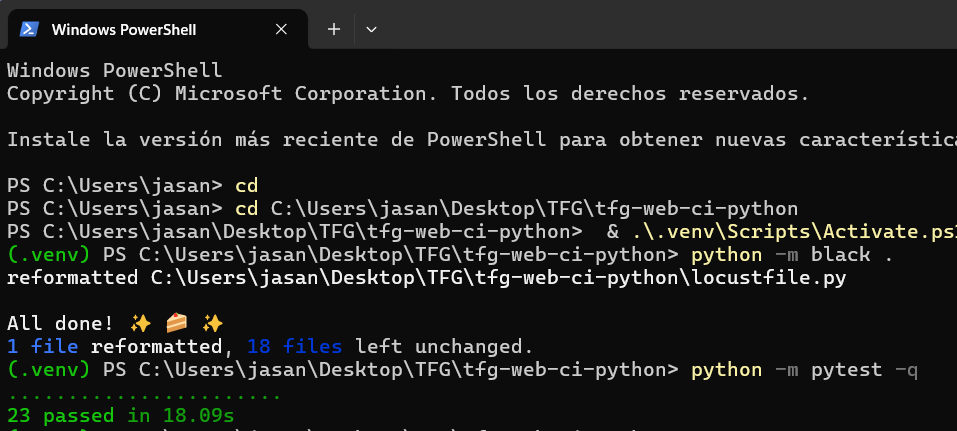
\includegraphics[width=0.86\textwidth]{figs/test_output.png}
    \caption{Captura ilustrativa de una ejecución satisfactoria de la validación automatizada en una fase previa del proyecto. Se mantiene como ejemplo visual del flujo de comprobación, aunque la validación final documentada del cierre alcanzó 29 pruebas superadas.}
    \label{fig:test_output_final}
\end{figure}

\section{Integración continua y validación sobre rama principal}

La validación técnica no se limitó a ejecuciones locales. Se reparó y estabilizó la configuración de \textbf{GitHub Actions}, de modo que la rama principal del proyecto quedara asociada a una comprobación automática de calidad. Este mecanismo permitió reforzar la confianza en el estado final de \texttt{main} tras la consolidación del rediseño y los hotfixes posteriores.

La utilidad de esta integración continua fue doble:

\begin{itemize}
    \item detectar con rapidez errores de formato, sintaxis o regresión;
    \item convertir la rama principal en una referencia técnica más fiable para cierre y entrega.
\end{itemize}

\section{Validación visual en Render}

Además de la validación automatizada, el proyecto requirió una validación visual manual sobre el entorno realmente desplegado. Para ello se utilizó Render como plataforma de ejecución en producción y se combinó un flujo de trabajo con rama de vista previa y rama principal.

Durante el rediseño frontend, la rama \texttt{bot/render-preview} se utilizó para revisar visualmente los cambios antes de su consolidación definitiva. Una vez cerradas las fases del rediseño y superadas las microcorrecciones finales, dichos cambios se integraron en \texttt{main}, que pasó a representar la versión oficial del producto.

La revisión visual se centró en las pantallas principales:

\begin{itemize}
    \item Home;
    \item Login y Registro;
    \item Aprender y readiness quiz;
    \item Modo Práctica;
    \item Modo Carrera;
    \item Modo Horizonte;
    \item Historial.
\end{itemize}

Esta validación permitió corregir jerarquía visual, inconsistencias entre botones, alineaciones, responsive intermedio y diferencias entre estados antes del cierre del proyecto.

\section{Validación con PostgreSQL y entorno Render}

La estabilización final también exigió validar el sistema con \textbf{PostgreSQL} en Render. Esta comprobación fue especialmente relevante tras la expiración de una base de datos anterior, que obligó a crear una nueva instancia y a confirmar que la aplicación seguía comportándose correctamente con persistencia real.

Las verificaciones realizadas sobre este entorno incluyeron:

\begin{itemize}
    \item registro e inicio de sesión de usuarios reales;
    \item persistencia del historial para usuario autenticado;
    \item diferenciación correcta entre invitado y registrado;
    \item acceso a sesiones del modo carrera;
    \item mantenimiento del comportamiento esperado tras reinicios y nuevos despliegues.
\end{itemize}

La comprobación satisfactoria de estos puntos permitió considerar resuelta la transición desde una base de datos previa caducada a una nueva configuración operativa en Render.

\section{Incidencia final de autenticación y corrección de navbar}

Una de las últimas incidencias funcionales detectadas en producción se produjo tras verificar el inicio de sesión real con la nueva base de datos. Se comprobó que la sesión autenticada existía y que el contenido de ciertas pantallas reconocía al usuario, pero la barra de navegación de páginas internas seguía mostrando acciones propias de usuario anónimo, como \textit{Iniciar sesión} y \textit{Crear cuenta}.

El análisis permitió determinar que el problema no estaba en la autenticación en sí misma, sino en la condición de renderizado utilizada por la navbar. La corrección consistió en dar prioridad explícita al identificador de usuario autenticado frente al posible estado de invitado, evitando que un usuario ya autenticado heredase elementos visuales del flujo anónimo.

Como refuerzo de esta corrección se añadieron pruebas de HTML renderizado sobre rutas internas reales:

\begin{itemize}
    \item \texttt{/nuevo-analisis}
    \item \texttt{/aprende}
    \item \texttt{/modo-carrera}
    \item \texttt{/modo-horizonte}
\end{itemize}

El resultado final fue la desaparición correcta de los botones \textit{Iniciar sesión} y \textit{Crear cuenta} en contexto autenticado, manteniendo al mismo tiempo el comportamiento esperado para usuarios invitados. Tras esta corrección, la validación completa volvió a cerrarse con \textbf{29 pruebas superadas}.

\section{Validación funcional del rediseño frontend}

La validación del rediseño no se redujo a una única revisión estética, sino que se planteó como un proceso iterativo de comprobación de coherencia visual y de uso. A lo largo de las distintas fases se revisaron formularios, jerarquía de pantallas, mensajes, comportamiento responsive, tablas y flujos de acceso. Este proceso hizo posible detectar problemas reales que no se apreciaban con la mera inspección de código, especialmente en el entorno desplegado.

Entre los aspectos verificados durante esta fase se encuentran:

\begin{itemize}
    \item coherencia entre pantallas principales;
    \item simplificación del acceso y la navegación;
    \item mejora del peso visual de los modos principales;
    \item organización más clara del modo carrera;
    \item integración prudente del modo horizonte;
    \item correcciones de responsive en anchuras intermedias y móviles.
\end{itemize}

La consolidación del rediseño en \texttt{main}, junto con el etiquetado \texttt{v1.1-frontend-redesign}, permitió cerrar esta fase con una referencia estable del estado visual del producto.

\section{Síntesis de resultados}

Tomando en conjunto la validación automatizada, la revisión sobre Render, la integración con PostgreSQL y la corrección de incidencias reales, puede afirmarse que el sistema alcanzó un estado final técnicamente consistente para el alcance de un TFG. Más allá del cumplimiento funcional básico, se consiguió un cierre razonable en términos de estabilidad, coherencia de interfaz y trazabilidad del proceso de mejora.
